\chapter{Prometheus} \label{chap:Prometheus}

\section{Cosa è?}
\textbf{Prometheus} è un framework di \textbf{monitoraggio} e di \textbf{alerting} che può essere utilizzato sia per il monitoraggio dello stato di salute di un cluster sia per il monitoraggio di una specifica applicazione. Sulle \textbf{metriche} prodotte è anche possibile applicare delle \textbf{regole} di alerting per segnalare eventuali criticità su diversi canali di comunicazione come email, slack, etc... \\
Inizialmente sviluppato da SoundCloud \cite{SoundCloud}, anche questo strumento è stato poi donato alla CNCF \cite{CNCF} e reso open source, diventando uno degli strumenti più diffusi nella sua categoria soprattutto grazie al suo \textbf{approccio modulare} che permette a chiunque lo desideri, di creare nuovi moduli per monitorare sistemi / strumenti / etc... non ufficialmente supportati.


\section{Metriche}
I dati utilizzati da Prometheus sono rappresentati sotto forma di metriche chiamate \textbf{time series}, composte da un \textbf{timestamp} relativo all'istante di collezionamento (nel tempo per una stessa metrica avremo più rilevamenti), e da coppie key-value opzionali dette \textbf{label} utilizzate per categorizzarle. \\
Queste time series possono essere facilmente interrogate e manipolate tramite l'apposito linguaggio di interrogazione detto \textbf{PromQL} \cite{Prometheus-query-language}, standardizzandone l'accesso e rendendo possibile interrogare tali metriche da diversi strumenti come la web UI di Prometheus, da richieste HTTP oppure tramite tool di terze parti come \textbf{Grafana} \cite{Grafana}. Grafana in particolare permette di creare \textbf{dashboard e grafi personalizzati} tramite un'apposita web UI, velocizzando la valutazione dello stato del sistema. 

\section{Architettura}
\begin{figure} [ht]
    \centering
    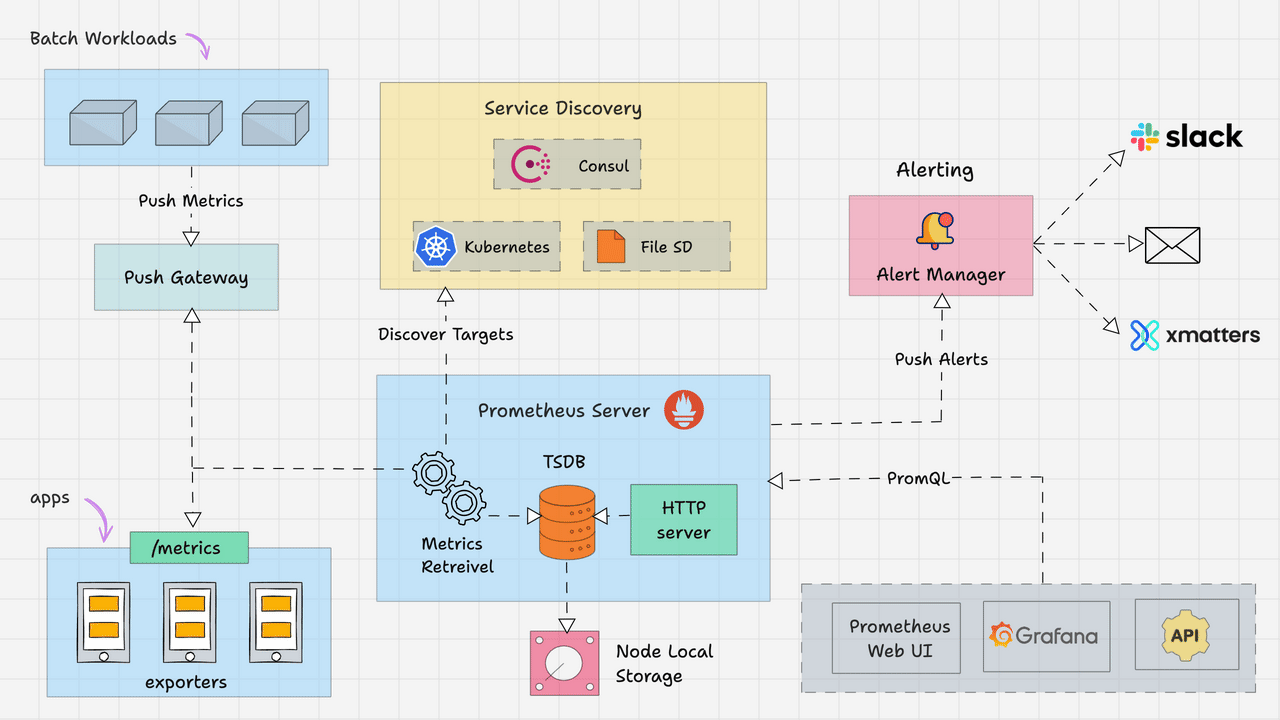
\includegraphics[width=1\linewidth]{UNINA_BSc_Final_Report//img//explanation/prometheus-architecture.png}
    \caption{architettura framework Prometheus \cite{Prometheus-architecture}}
    \label{fig:prometheus-architecture}
\end{figure}
L'approccio utilizzato da Prometheus per recuperare i dati è detto \textbf{scraping}, che sarà approfondito a breve, mentre i dati come già detto sono rappresentati sotto forma di metriche.\\ 
L'architettura si può suddividere nelle seguenti componenti, considerabili come moduli a se stanti [fig. \ref{fig:prometheus-architecture}]: \\

\begin{itemize}
    \item \textbf{Server} \\
    cuore di questo strumento, colleziona le metriche dai vari target con un pattern pull, periodicamente tramite richieste HTTP (processo detto \textbf{scraping}), dove il periodo di tempo può essere personalizzato. E' composto a sua volta da:
    \begin{itemize} 
        \item \textbf{Time-Series Database (TSDB)}: database che immagazzina le time series delle metriche in maniera persistente ed efficiente, sfruttando apposite policy temporali per la conservazione; di default salva i dati in locale sul nodo in cui viene installato Prometheus, ma può essere configurato per il salvataggio in cloud.
        \item \textbf{HTTP server}: abilita l'interrogazione al TSDB tramite richieste HTTP ricevute dall'esterno contenenti le query in \textit{PromQL}.
        \item \textbf{Metrics Retrieval}: colleziona le metriche dai \textbf{target} inviando richieste HTTP periodicamente.
    \end{itemize}

    \item \textbf{Targets} \\
    sorgenti per lo scraping del server, in genere utilizzano degli \textbf{exporter} che convertono delle metriche da un formato non supportato (per esempio metriche di sistema) ad uno adatto a Prometheus, o delle \textbf{librerie cliente} che permettono di esporre delle metriche personalizzate da un applicazione scrivendo direttamente nel codice. Entrambe queste tipologie di moduli possono essere creati da zero da qualsiasi utente, per questo le loro liste vengono suddivise in ufficiali e non \cite{Prometheus-clients-exporters-list}. \\
    Negli scenari in cui non è possibile utilizzare il pattern pull come in task di breve durata, allora si può utilizzare il \textbf{PushGateway}, un componente a se stante che funge da buffer temporaneo, permettendo ai target di inviare direttamente le metriche (pattern \textbf{push}) a quest'ultimo, dalla quale saranno poi estratte come in un target classico.

    \item \textbf{Service Discovery} \\
    uno dei concetti principali di questo strumento, i target possono essere rilevati in 2 modi: 
    \begin{itemize} 
        \item \textbf{configurazione statica}: i target sono hard coded nei file di configurazione di Prometheus o in appositi file YAML/Json, ma ciò è possibile solo con target che hanno endpoint statici, che in genere non è nella natura degli oggetti di Kubernetes.
        \item \textbf{Sevice Discovery}: consente a Prometheus di rilevare e monitorare automaticamente i target senza richiedernee la configurazione manuale per ognuno di essi.
    \end{itemize}

    \item \textbf{Alert Manager} \\
    per quanto riguarda l'alerting, Prometheus si occupa unicamente di \textbf{triggerare} gli alert definendo delle \textbf{treshold}, ma tali alert sono poi gestiti dall'\textbf{Alert Manager}, il quale dopo averci effettuato diverse manipolazioni come la decuplicazione, raggruppamento, etc... notificherà gli appositi destinatari in base ai diversi criteri di \textbf{routing} con il quale è stato configurato.
    
\end{itemize}

\section{Prometheus Operator} 
Per installare Prometheus si possono usare 2 approcci principalmente, uno \textbf{classico} installando il framework come una normale applicazione usando dei file binari pre-compilati, delle immagini Docker o Helm, dove però è richiesto un processo di configurazione lento e tedioso consistente nella creazione e modifica di diversi file di configurazione in maniera statica, aumentando di molto i tempi di setup ed eventualmente di troubleshooting. \\
Invece, un altro approccio che si può utilizzare è quello di sfruttare gli \textbf{operatori} di Kubernetes, che potremo dire essere la nuova frontiera per la distribuzione di applicazioni in un cluster, infatti gli operatori non sono altro che delle \textbf{estensioni} che permettono di integrare un'applicazione in maniera più stretta con Kubernetes, dando così la possibilità di creare degli \textbf{oggetti personalizzati} utilizzando delle \textbf{Custom Resource Definitions} (CRDs). 
\\
Prometheus mette a disposizione il \textbf{Prometheus Operator} \cite{Prometheus-operator}, che consente di installare in modo semplice l'intero stack di monitoraggio (Prometheus, Alert Manager, Grafana, etc.), semplificando significativamente la configurazione del framework. Grazie a questo strumento, non è più necessario modificare manualmente i file di configurazione, ma si possono invece creare oggetti personalizzati, come il Deployment di Prometheus o dell'Alert Manager. La configurazione può essere suddivisa in più oggetti personalizzati distinti, evitando l'uso di un unico file. Ad esempio, il ServiceMonitor permette di dichiarare quali servizi di Kubernetes monitorare, migliorando la modularità e la gestione della configurazione. \\
Tutto ciò avviene semplicemente installando il Prometheus Operator e creando nuovi oggetti personalizzati, che verranno automaticamente rilevati tramite l'uso delle label, aggiornando automaticamente tutte le configurazioni che in passato avrebbero richiesto interventi manuali.

\section{Sistema locale}

Come già anticipato per comprendere al meglio il funzionamento di tali strumenti, è stato ricreato un ambiente simile a quello utilizzato nella campagna di fault/error injection con un'applicazione campione [fig. \ref{fig:local-cluster}], con ovvie limitazioni a causa della disponibilità di risorse computazionali. 

\begin{figure} [ht]
    \centering
    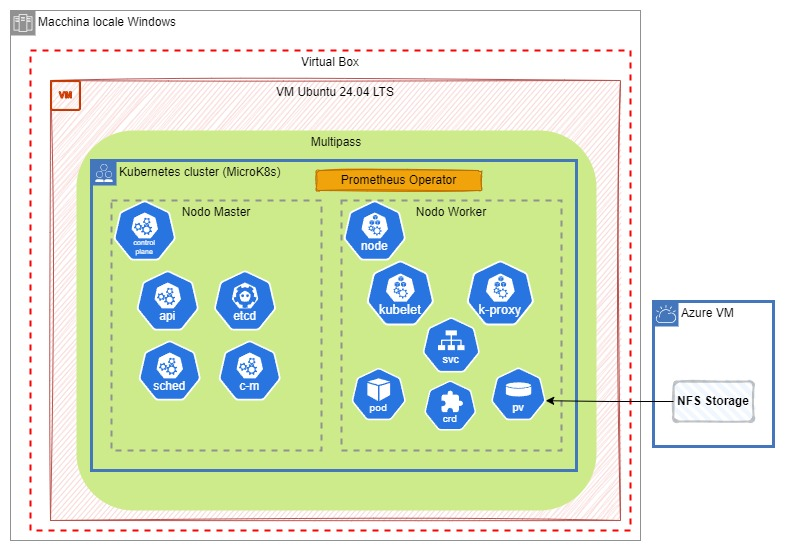
\includegraphics[width=1\linewidth]{UNINA_BSc_Final_Report//img//explanation/local_environment.jpg}
    \caption{infrastruttura cluster locale}
    \label{fig:local-cluster}
\end{figure}

\subsection{Ambiente}
Partendo dall'alto verso il basso il sistema gira su una macchina virtuale Ubuntu 24.04 LTS \cite{Ubuntu} eseguita su VirtualBox 7.0.20 \cite{VirtualBox}, con 4 core e circa 10 GB di memoria. \\
Su tale VM gira l'intero cluster, composto da 2 nodi (1 master e 1 worker), dove ogni nodo corrisponde a sua volta ad un altra macchina virtuale Ubuntu 24.04 LTS da 1 core e 4 GB di memoria, gestite con Multipass 1.14.0 \cite{Multipass}.

\subsection{MicroK8s}
Per creare un cluster Kubernetes è stato utilizzato \textbf{MicroK8s} 1.30.0 \cite{MicroK8s}, framework open source che permette di creare un \textbf{cluster lite} adatto a sistemi con poche risorse. \\
Il vero vantaggio di tale framework però è nella \textbf{semplicità} della configurazione del cluster, il punto debole di Kubernetes, infatti MicroK8s permette di creare un cluster semplicemente installando il framework su ogni nodo (ad esempio con \textbf{Snap} \cite{Snap}), utilizzare un apposito comando dal nodo master e copiare ed incollare le istruzioni a schermo sui nodi worker, ed il cluster è già configurato. \\
Un altre grande vantaggio di MicroK8s sono gli \textbf{addon}, ovvero delle estensioni attivabili direttamente tramite MicroK8s già preconfigurate e pronte all'uso, in particolare è stato abilitato l'addon \textbf{observability} che permette di installare lo stack \textbf{Kube-prometheus} \cite{Kube-prometheus}, che comprende il Prometheus Operator, Grafana, l'Alert Manager e un insieme di exporter per monitorare lo stato del cluster come Kube-state-metrics \cite{Kube-state-metrics} e node-exporter \cite{Node-exporter}. Anche in questo caso con un semplice comando da terminale \textit{microk8s enable observability}, l'intero ecosistema di Prometheus è già in funzione per monitorare lo stato del cluster con anche delle regole di alerting predefinite.

\subsection{Applicazione campione}
Come applicazione da monitorare è stata scelta un'applicazione per la gestione di sensori di temperatura e pressione, costituita da un BE in Flask e da degli script per simulare le richieste dei client \footnote{Il codice è disponibile su GitHub \cite{github-repo}, mentre le immagini dei container su DockerHub \cite{docker-images}}.
Oltre a monitorare lo stato del cluster, è stata modificata l'applicazione utilizzando una delle client library di Prometheus permettendo di aggiungere l'endpoint per lo scraping e realizzare delle metriche personalizzate [fig. \ref{fig:flask-be}] per monitorare le richieste ricevute, il tempo di elaborazione e le relative risposte.


\begin{figure} [ht]
    \centering
    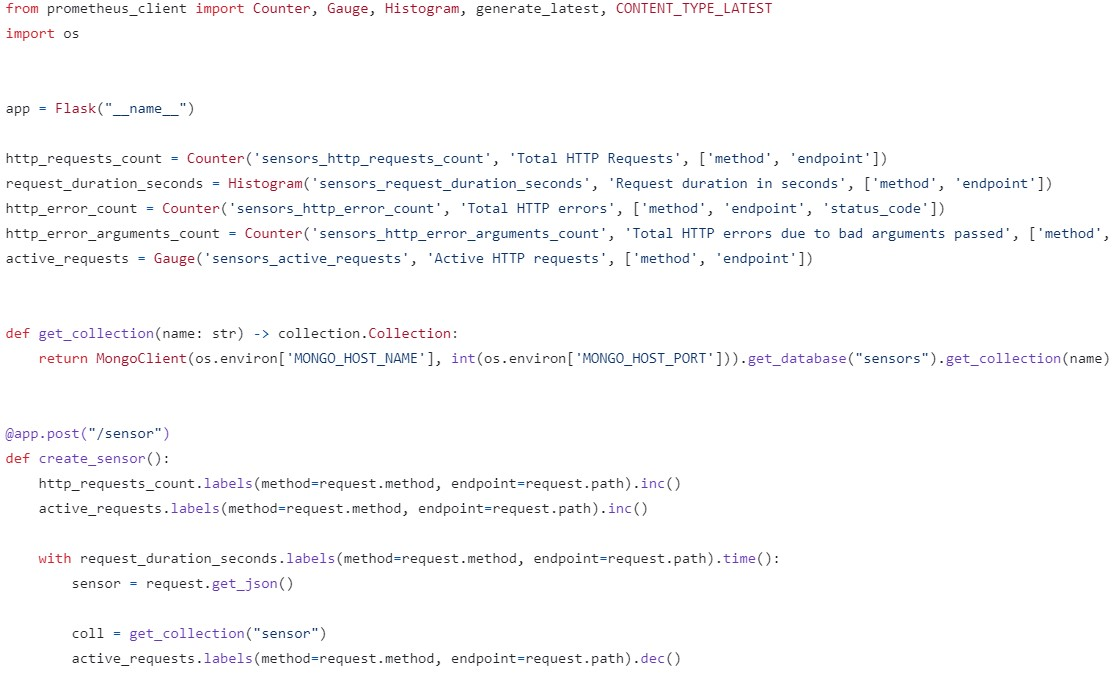
\includegraphics[width=0.95\linewidth]{UNINA_BSc_Final_Report//img//explanation/controller_example.jpg}
    \caption{esempio BE Flask con metriche da client library}
    \label{fig:flask-be}
\end{figure}

\subsection{Configurazione applicazione campione}
Per poter monitorare anche l'applicazione d'esempio è necessario creare degli appositi oggetti di Kubernetes \footnote{Tutti i file per creare questi oggetti sono disponibili sul repository GitHub \cite{github-repo} in formato .yaml.} , sia per quanto riguarda la gestione dell'applicazione che per configurare Prometheus ad effettuare lo scraping delle nuove metriche.

\subsubsection{Deployment applicazione}
Il deploy dell'applicazione è costituito dai seguenti oggetti Kubernetes:
\begin{itemize}
    \item \textbf{Deployment} del BE in Flask.
    \item \textbf{Service} \footnote{I Service sono degli oggetti di Kubernetes che si occupano di rendere disponibile in rete determinati pod, selezionati ad esempio tramite label, e fare loro da load balancer.} per esporre il BE all'esterno.
    \item \textbf{StatefulSet} per l'istanza di MongoDB.
    \item \textbf{Service} per esporre MongoDB al BE.
    \item \textbf{PersistentVolume} per rendere persistenti i dati di MongoDB, utilizzando una macchina virtuale su Azure come NFS storage.
    \item \textbf{Deployment} per gli script dei client.
\end{itemize}

\subsubsection{Configurazione Prometheus}
La configurazione di Prometheus è avvenuta in maniera analoga a quanto fatto precedentemente grazie al Prometheus Operator, con il quale è stato sufficiente creare degli \textbf{oggetti personalizzati} per tale operatore senza dover toccare i file di configurazione di Prometheus stesso. Per fare ciò è stato sufficiente creare un numero ridotto di oggetti sfruttando gli oggetti già creati dall'addon observability, impostando le \textbf{label} dei nuovi oggetti in maniera opportuna per far funzionare correttamente il \textbf{service discovery} di Prometheus. In particolare:
\begin{itemize}
    \item \textbf{Service} per esporre Prometheus, Grafana e l'Alert Manager all'esterno.
    \item \textbf{ServiceMonitor} per abilitare il monitoraggio (scraping) al Service del BE.
    \item \textbf{PrometheusRule} per creare un'alert rule personalizzata campione.
\end{itemize}

Con questa configurazione possiamo sia monitorare lo stato del cluster sfruttando gli exporter e le dashboard preinstallate [fig. \ref{fig:grafana-cluster}] o sfruttando metriche e dashboard personalizzate [fig. \ref{fig:grafana-sensor}], sia applicare delle regole di alerting in pochi semplici passaggi.
\\
\begin{figure} [ht]
    \centering
    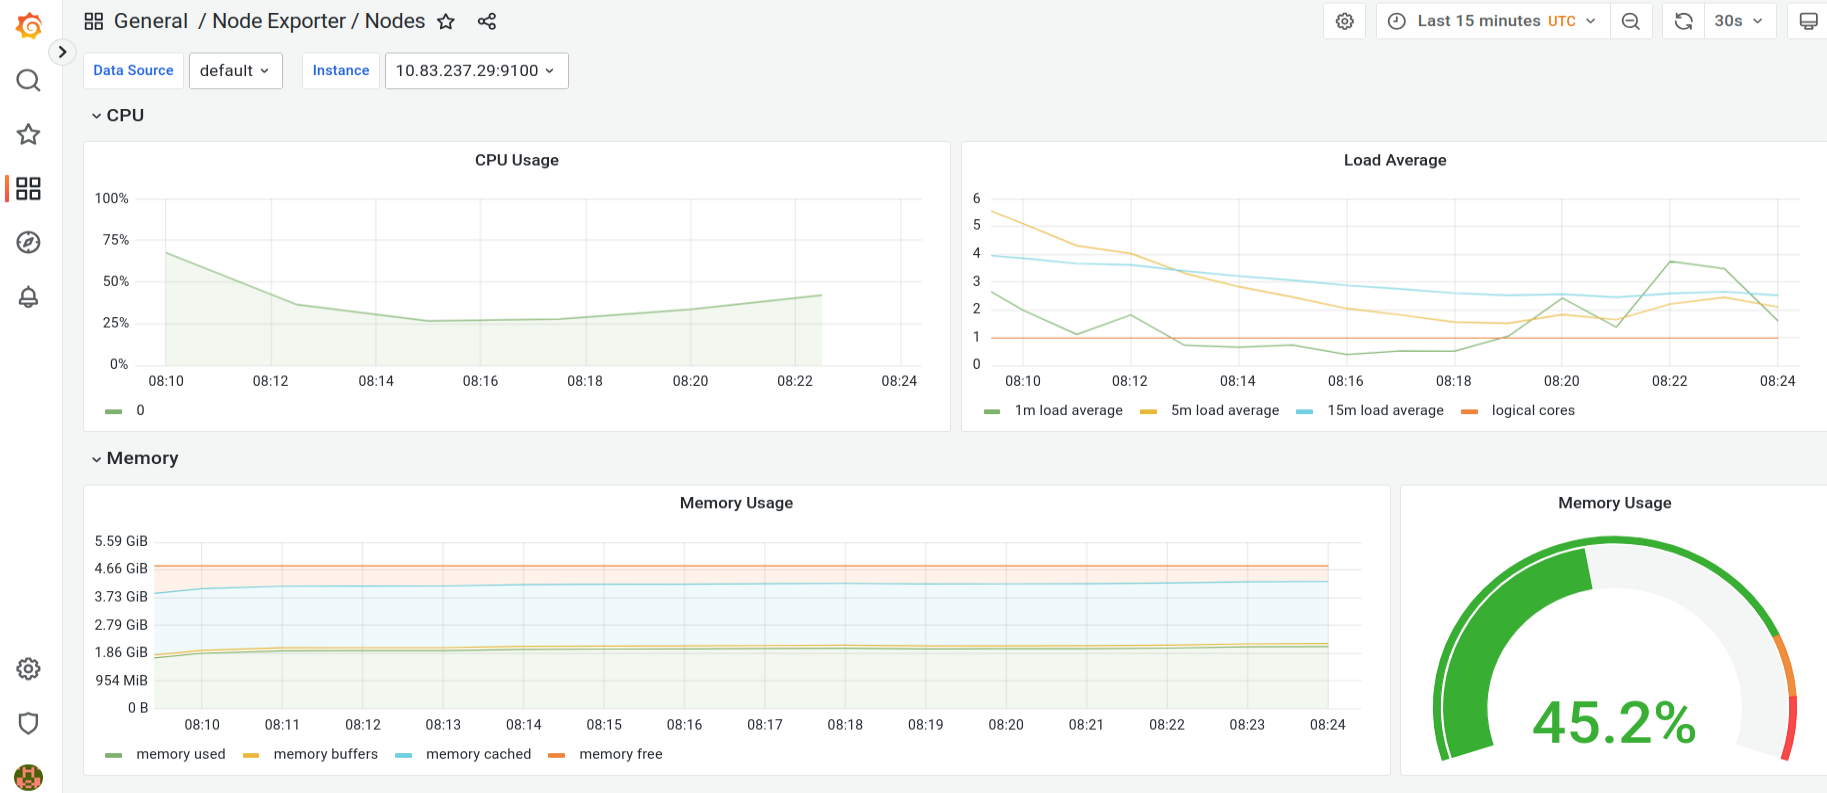
\includegraphics[width=1\linewidth]{UNINA_BSc_Final_Report//img//explanation/grafana_example_white.png}
    \caption{dashboard Grafana con metriche da Node Exporter}
    \label{fig:grafana-cluster}
\end{figure}

\begin{figure} [ht]
    \centering
    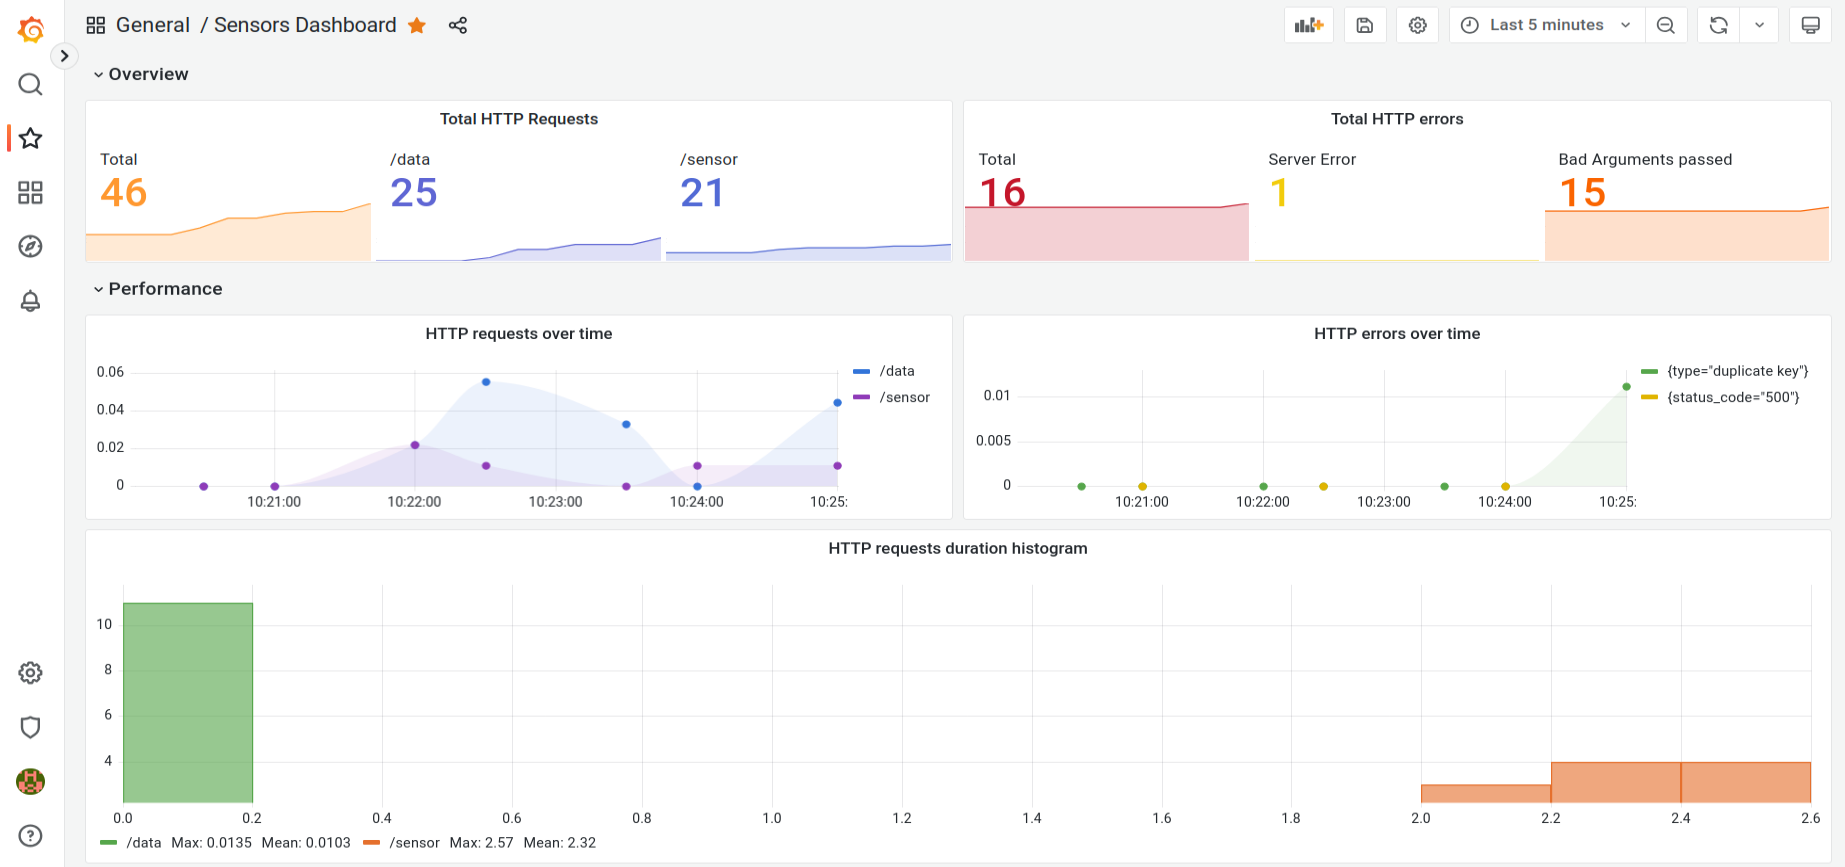
\includegraphics[width=1\linewidth]{UNINA_BSc_Final_Report//img//explanation/grafana_sensor_example_white.png}
    \caption{dashboard Grafana personalizzata del BE}
    \label{fig:grafana-sensor}
\end{figure}